

\tikzset{every picture/.style={line width=0.3pt}} %set default line width to 0.75pt        

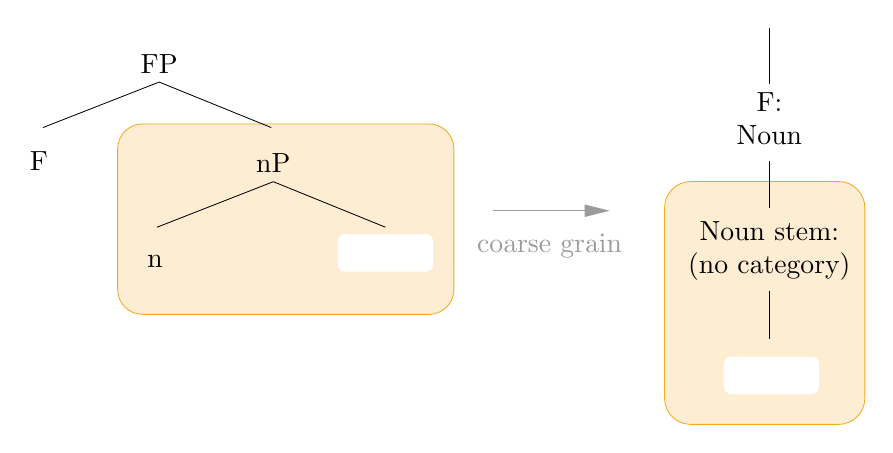
\begin{tikzpicture}[x=0.75pt,y=0.75pt,yscale=-1,xscale=1]
%uncomment if require: \path (0,300); %set diagram left start at 0, and has height of 300

%Rounded Rect [id:dp7624647334912189] 
\draw  [color={rgb, 255:red, 245; green, 166; blue, 35 }  ,draw opacity=1 ][fill={rgb, 255:red, 245; green, 166; blue, 35 }  ,fill opacity=0.2 ] (341.5,104.55) .. controls (341.5,97.58) and (347.15,91.93) .. (354.12,91.93) -- (425.38,91.93) .. controls (432.35,91.93) and (438,97.58) .. (438,104.55) -- (438,196.31) .. controls (438,203.28) and (432.35,208.93) .. (425.38,208.93) -- (354.12,208.93) .. controls (347.15,208.93) and (341.5,203.28) .. (341.5,196.31) -- cycle ;
%Rounded Rect [id:dp5385241045114268] 
\draw  [color={rgb, 255:red, 245; green, 166; blue, 35 }  ,draw opacity=1 ][fill={rgb, 255:red, 245; green, 166; blue, 35 }  ,fill opacity=0.2 ] (78,76.18) .. controls (78,69.55) and (83.37,64.18) .. (90,64.18) -- (228,64.18) .. controls (234.63,64.18) and (240,69.55) .. (240,76.18) -- (240,143.93) .. controls (240,150.55) and (234.63,155.93) .. (228,155.93) -- (90,155.93) .. controls (83.37,155.93) and (78,150.55) .. (78,143.93) -- cycle ;
%Rounded Rect [id:dp9718477695197401] 
\draw  [draw opacity=0][fill={rgb, 255:red, 255; green, 255; blue, 255 }  ,fill opacity=1 ] (184,120.85) .. controls (184,118.85) and (185.62,117.23) .. (187.61,117.23) -- (226.39,117.23) .. controls (228.38,117.23) and (230,118.85) .. (230,120.85) -- (230,131.69) .. controls (230,133.69) and (228.38,135.3) .. (226.39,135.3) -- (187.61,135.3) .. controls (185.62,135.3) and (184,133.69) .. (184,131.69) -- cycle ;
%Straight Lines [id:da6007728522572746] 
\draw    (153,92) -- (207,113.93) ;
%Straight Lines [id:da04101278854045498] 
\draw    (153,92) -- (97,113.93) ;
%Straight Lines [id:da015472500413207468] 
\draw [color={rgb, 255:red, 155; green, 155; blue, 155 }  ,draw opacity=1 ]   (259,106) -- (313,106) ;
\draw [shift={(315,106)}, rotate = 180] [fill={rgb, 255:red, 155; green, 155; blue, 155 }  ,fill opacity=1 ][line width=0.08]  [draw opacity=0] (12,-3) -- (0,0) -- (12,3) -- cycle    ;
%Straight Lines [id:da08471453499162984] 
\draw    (98,44) -- (152,65.93) ;
%Straight Lines [id:da2431991859779299] 
\draw    (98,44) -- (42,65.93) ;
%Straight Lines [id:da5826203844696023] 
\draw    (392,18) -- (392,44.93) ;
%Straight Lines [id:da13455897274706574] 
\draw    (392,81.93) -- (392,104.85) ;
%Straight Lines [id:da2602172842725583] 
\draw    (392,144.85) -- (392,167.78) ;
%Rounded Rect [id:dp7345999015639559] 
\draw  [draw opacity=0][fill={rgb, 255:red, 255; green, 255; blue, 255 }  ,fill opacity=1 ] (370,179.85) .. controls (370,177.85) and (371.62,176.23) .. (373.61,176.23) -- (412.39,176.23) .. controls (414.38,176.23) and (416,177.85) .. (416,179.85) -- (416,190.69) .. controls (416,192.69) and (414.38,194.3) .. (412.39,194.3) -- (373.61,194.3) .. controls (371.62,194.3) and (370,192.69) .. (370,190.69) -- cycle ;

% Text Node
\draw (153,89) node [anchor=south] [inner sep=0.75pt]   [align=left] {nP};
% Text Node
\draw (96,134.77) node [anchor=south] [inner sep=0.75pt]   [align=left] {n};
% Text Node
\draw (250,116) node [anchor=north west][inner sep=0.75pt]  [color={rgb, 255:red, 155; green, 155; blue, 155 }  ,opacity=1 ] [align=left] {coarse grain};
% Text Node
\draw (40,87.77) node [anchor=south] [inner sep=0.75pt]   [align=left] {F};
% Text Node
\draw (98,41) node [anchor=south] [inner sep=0.75pt]   [align=left] {FP};
% Text Node
\draw (392,47.93) node [anchor=north] [inner sep=0.75pt]   [align=left] {\begin{minipage}[lt]{26.8pt}\setlength\topsep{0pt}
\begin{center}
F:\\Noun
\end{center}

\end{minipage}};
% Text Node
\draw (392,109.85) node [anchor=north] [inner sep=0.75pt]   [align=left] {\begin{minipage}[lt]{62.48pt}\setlength\topsep{0pt}
\begin{center}
Noun stem:\\(no category)
\end{center}

\end{minipage}};


\end{tikzpicture}
